\begin{figure}[htp]
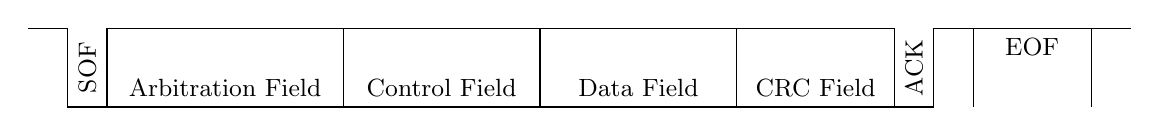
\begin{tikzpicture}
	%SOF
	\draw (0,1) -- ++(0.5,0) -- ++(0,-1) -- ++(0.5,0) -- ++(0,1);
	\node[rotate=90] at (0.75,0.5) {\small SOF};
	%Arbitration Field
	\draw (1,1) -- ++(3, 0);
	\draw (1,0) -- ++(3, 0) node[midway, above=0.25] {\small Arbitration Field};
	\draw (4, 0) -- ++(0,1);
	%Control Field
	\draw (4,1) -- ++(2.5, 0);
	\draw (4,0) -- ++(2.5, 0) node[midway, above=0.25] {\small Control Field};
	\draw (6.5, 0) -- ++(0,1);
	%Data Field
	\draw (6.5,1) -- ++(2.5, 0);
	\draw (6.5,0) -- ++(2.5, 0) node[midway, above=0.25] {\small Data Field};
	\draw (9, 0) -- ++(0,1);
	%CRC Field
	\draw (9,1) -- ++(2, 0);
	\draw (9,0) -- ++(2, 0) node[midway, above=0.25] {\small CRC Field};
	\draw (11, 0) -- ++(0,1);
	%ACK Field
	\draw (11,0) -- ++(0.5,0);
	\draw (11.5,0) -- ++(0,1);
	\node[rotate=90] at (11.25,0.5) {\small ACK};
	\draw (11.5,1) -- ++(0.5,0);
	\draw (12,0) -- ++(0,1);
	%EOF
	\draw (12,1) -- ++(1.5, 0) node[midway, below=0.25] {\small EOF};
	\draw (13.5, 0) -- ++(0,1);
	\draw (13.5,1) -- ++(0.5,0);

\end{tikzpicture}
\caption{CAN Frame Format}
\label{fig:can_frame_format}
\end{figure}